%TC:envir lstlisting [] xall

\definecolor{purple}{rgb}{0.65, 0.12, 0.82}
\lstset{
	breakatwhitespace=true,
	breaklines=true,
	keywordstyle=\color{blue}\bfseries,
	identifierstyle=\color{black},
	commentstyle=\color{purple}\itshape,
	stringstyle=\color{red},
	float=here
}

\lstdefinelanguage{javascript}{
	keywords={break, case, catch, continue, debugger, default, delete, do, else, false, finally, for, function, if, in, instanceof, new, null, return, switch, this, throw, true, try, typeof, var, void, while, with},
	morecomment=[l]{//},
	morecomment=[s]{/*}{*/},
	morestring=[b]',
	morestring=[b]",
	ndkeywords={class, export, boolean, throw, implements, import, this},
	sensitive=true
}
\chapter{Application Implementation}

This chapter details how the application was implemented, listing the technologies, frameworks and coding methods used. It looks at all parts of the application, from the article discovery system to the methods used for obtaining the translations and grammatical information used in the gloss, detailing the implementation of each feature. Parts of the source code are used throughout, to show in detail how these feature were implemented and then integrated with the rest of the application. A copy of the entire source code of the application can be found in the design archive.

\section{General Technologies and Frameworks}

As it is a web application, HTML, CSS and JavaScript were used for the client side of the application, although this was augmented with both \textit{JQuery} and \textit{Bootstrap} to ease the development of the Javascript and the CSS respectively. 

For the server side of the application, the code was written in Python, using the \textit{Flask} framework and its integrated technologies. \textit{Flask} was used as it is easier to use then the alternative Python frameworks and the developer has experience using it. Python was also chosen for similar reasons, including the developer's experience with it. The memory usage and speed of the various possible programming languages and frameworks was not considered. Ease of use and familiarity were the primary concerns. 

\section{Article Discovery}

For the article discovery portion of the application, the need was for a list of articles, from a variety of sources about a variety of topics. The solution that was found after some searching on the internet, was \textit{Google News}.

\textit{Google News} provides several lists of recent articles from different sources divided in different topics, additionally, each of these lists is provided in an RSS feed XML file, a format that allows the code to be written for both URL and title extraction with minimal effort.

The categories provided by the \textit{Google News} RSS feeds were usable, but overall they were fairly common news categories. On the plus side, these categories are recognisable, on the down side, these categories are not customisable, but the categories were pre-selected, saving time on artificial category creation, the end user can just select one of them. The code for obtaining the articles is shown in Listing \ref{lst:disc}.

\begin{lstlisting}[caption={[Article Discovery Code] Python code for obtaining news articles from the \textit{Google News} RSS feeds.}, label=lst:disc, language=python, float]
    # get the articles in a category
    def lookup(self, category, user_level):

        # get the rss feed
        r = requests.get(CAT_MAP[category]['url'])
        root = ElementTree.fromstring(r.text)

        # get the old articles from memory
        old_aritcles = [a.id for a in self.articles[category]]

        # iterate through the article in the rss feed, extracting the articles
        for item in root.iter('item'):
            url = item.find('link').text
            title = item.find('title').text
            aid = str(uuid.uuid5(uuid.NAMESPACE_URL, url))

            # if the article is not already saved, try to parse and rate it (some articles fail)
            if aid not in old_aritcles:
                try:
                    self.articles[category].append(Article(url, title, aid, category))
                except ZeroDivisionError:
                    print('Zero Divison Error')
                except ArticleException:
                    print('Article Exception')

        # return the list of articles classified.
        return self.classify(self.articles[category], user_level)
\end{lstlisting}


This code takes the category, and then gets the current state of the corresponding RSS feed. It then iterates through item tags in the RSS feed, extracting the title and URL of each tag. It then attempts to parse and rate the article for listing. Once every article has be parsed and rated, it returns a list for display. In addition, articles are stored and added to future lists so that the code doesn't have to reparse an article every time the list is generated.

There were alternatives to the \textit{Google News} RSS feeds that were examined, primarily \textit{NewsAPI}. However this was found to be lacking for two reasons. Primarily, this API would list content, where the primary means of communication was not text. Comics and other image-based media got added to the lists being provided by the API. As the parser and the gloss system relied on the content being text based and there was no easy way to distinguish between text based content and image based content. The other more minor reason that \textit{NewsAPI} was disregarded was because it was more difficult to categorise the articles, whereas the \textit{Google News} RSS feeds provided pre-created categories, to save time on both filtering out image-based content and the categorisation of articles, the decision was made to use the \textit{Google News} RSS feeds. 


\section{Article Difficulty Rating}

The difficulty rating of the article is calculated using two things, the article text as well as the user's experience level. The user's experience level is obtained from the form the user submitted at the start, while the article text needs to be extracted from the article web page and then analysed.

To extract and then analyse the article, two technologies are used. The first is an article scraping Python library called \textit{Newspaper}, the purpose of it is to extract the raw article text from the article web page, making the analysis of it easier. Analysis of the article text is then done through another P ython library called \textit{SpaCy}, which is a parts-of-speech tagging library, while an add-on for it, called \textit{Textacy} provides advanced features such as syllable counting. \textit{SpaCy} provides two  sets of parts-of-speech tags with different levels of precision, which are referred to as fine-grained and coarse-grained, with fine-grained being the more precise one, while coarse-grained is less precise, it has advantage of being functionally identical to the lexical category of a given word.

Once the article text has been extracted and analysed, it's readability index needs to be calculated, this is done using the Erste Wiener Sachetextformel (WSTF) as described in \textcite{bamberger1984}. The WSTF formula was chosen over the FRE formula because the WSTF formula has a smaller output range. This smaller output range allowed for two things the first was easier mapping onto the user experience level as well as a better understanding of the approximate level of each individual number, as those number correspond directly with the German school years. 

Once the readability score is calculated, it needs to be mapped, using the user experience level onto the difficulty ratings, a simple linear map was chosen for this, the mappings can be seen in Figure \ref{fig:ratings}.

\begin{figure}
	\caption[Aritcle Rating Mappings]{Mappings showing the article readability score against experience level and the ratings decided upon based on those variables.}
	\label{fig:ratings}
	\begin{center}
	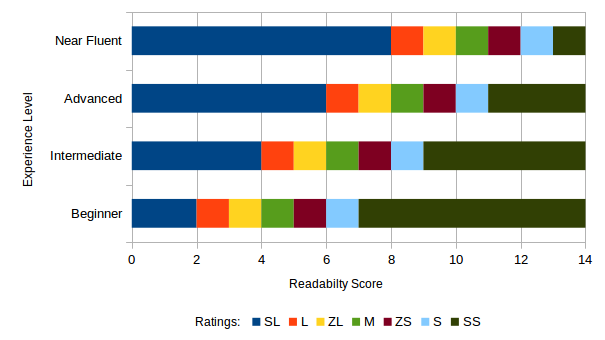
\includegraphics[width=0.7\textwidth]{Graphics/Ratings}
\end{center}
\end{figure}

The primary idea behind these ratings was that the threshold between the difficulty ratings would be lower for less experienced users, but that the range of scores within the ratings would be approximately the same, as the readability score scales with experience. Once this was decided, a reference point was needed to decide the ratings. A near fluent user should be able to read with some confidence articles with a WSTF score of 10, which corresponds to a native speaker who is 15/16 years old. The rest of the mappings were then extrapolated from there. 

More complex ideas for mapping were experimented with, including ones that used machine learning systems. These ideas were eventually abandoned due to the fact that they were too complex to be implemented in the limited time available. 

\section{Displaying the Article}

Once the users has selected an article, they are then presented with the content of that article. The actual job of presenting this article was fairly easy as the majority of this work (the extraction and parsing of the article's content) had already been done by \textit{newspaper} and \textit{SpaCy}. \textit{SpaCy's} method of presenting the parsed article is as a series of parts-of-speech tags. This makes presenting the article easy, the tags are iterated through as if they were a list. Words are wrapped in span elements tags for later use, punctuation is outputted without these tags and a paragraph break in the text starts a new paragraph in the HTML. In addition the span tags used for words have data attributes storing the parts-of-speech tags and root word. This results in a html document that appears similar to Listing \ref{lst:html}.

\begin{lstlisting}[language=HTML, caption=Example HTML Code, label=lst:html, breaklines=true]
<p>
	<span class="word" data-lemma="Der" data-tag="ART" data-pos="DET">Der</span>
	<span class="word" data-lemma="Index" data-tag="NN" data-pos="NOUN">Index</span>
	<span class="word" data-lemma="der" data-tag="ART" data-pos="DET">der</span>
	<span class="word" data-lemma="30" data-tag="CARD" data-pos="NUM">30</span>
	<span class="word" data-lemma="groß" data-tag="ADJA" data-pos="ADJ">größten</span>
	<span class="word" data-lemma="Aktiengesellschaften" data-tag="NN" data-pos="NOUN">Aktiengesellschaften</span>
	<span class="word" data-lemma="steigen" data-tag="VVFIN" data-pos="VERB">stieg</span>
	<span class="word" data-lemma="heute" data-tag="ADV" data-pos="ADV">heute</span>
	<span class="word" data-lemma="zeitweise" data-tag="ADV" data-pos="ADV">zeitweise</span>
	<span class="word" data-lemma="bis" data-tag="APPR" data-pos="ADP">bis</span>
	<span class="word" data-lemma="auf" data-tag="ADV" data-pos="ADV">auf</span>
	<span class="word" data-lemma="12.524,97" data-tag="CARD" data-pos="NUM">12.524,97</span>
	<span class="word" data-lemma="punkten" data-tag="NN" data-pos="NOUN">Punkte</span>
	,
	<span class="word" data-lemma="entsprechen" data-tag="ADJD" data-pos="ADJ">entsprechend</span>
	<span class="word" data-lemma="einer" data-tag="ART" data-pos="DET">einem</span>
	<span class="word" data-lemma="gewinnen" data-tag="NN" data-pos="NOUN">Gewinn</span>
	<span class="word" data-lemma="von" data-tag="APPR" data-pos="ADP">von</span>
	<span class="word" data-lemma="0,13" data-tag="CARD" data-pos="NUM">0,13</span>
	<span class="word" data-lemma="Prozent" data-tag="NN" data-pos="NOUN">Prozent</span>
	.
</p>

\end{lstlisting}

The html produced by this was functional, although there was a bug to do with the generation of excess white-space, which was removed from Listing \ref{lst:html} so that the code was readable. 

\section{Gloss Creation}

The client side method for creating the gloss is done through AJAX, the JavaScript for this can be seen in Listing \ref{lst:gloss}.



\begin{lstlisting}[caption={[Gloss Javascript] Javascript/JQuery code for obtaining gloss content from the server and then inserting it into the web page.}, label=lst:gloss, language=javascript, float]
$('.word').on('click', function (event) {
	var e = event.target;
	var data = e.dataset;
	data.word = e.textContent;
	$.ajax({
		url: "/dict",
		type: 'POST',
		data: data,
		success: function (result) {
			popupEntry(result);
		}
	});
});

function popupEntry(entry) {
	var entryList = document.getElementById("dict-entries");
	entryList.insertAdjacentHTML('beforeend', entry);
}

\end{lstlisting}

This code is simple, when one of the words is clicked, an AJAX event is fired. It requests the gloss item from the application, and upon return inserts the gloss item at the end of the marginal gloss.

Upon receiving such a gloss request, the server side python code will then generate and return a pre-formatted gloss. This allowed for the client side code to be kept as simple as possible. The code for this gloss generation process is shown in Listing \ref{lst:dict}.

\begin{lstlisting}[caption=Gloss Generation Code, label=lst:dict, breaklines=true, language=python]
class DictEntry:
    def __init__(self, word, lemma, tag):
        self.word = word
        self.root = lemma
        self.tag = tag
        self.pos = TAG_DICT[tag]
        if self.pos in ['Noun', 'Verb', 'Adjective', 'Unknown']:
            self.css_cat = self.pos.lower()
        else:
            self.css_cat = 'other'

        if self.pos not in ['Proper Noun', 'Other', 'Numeral']:
            self.found, translation, grammar = dictionary.lookup(word, lemma, self.pos)
            if self.found:
                self.english = self.gen_english_string(translation)
                self.grammar_features = self.list_features(grammar)
            else:
                self.english = 'No translation found'
                self.grammar_features = []

        else:
            self.found = False
            self.english = 'Not translatable'
            self.grammar_features = []
        self.grammar_explanation = spacy.explain(tag)
\end{lstlisting}


The code starts by assigning the word, root and fine-grained parts-of-speech tag to the class, the fine-grained parts-of-speech tag is then used to lookup the lexical category, which is then saved in a human readable format.  If the lexical category is one where a translation will not be found (Proper Nouns, Numerals, etc.) then the code does not bother performing the lookups. For all other lexical categories, the code then calls the dictionary object (defined outside of scope) and looks up the translations of the word and its grammatical information. When this information is returned, it then proceeds to format it so it is human readable.

The object where all this has been stored is then passed to the template engine, where it is transformed into a HTML gloss item. This is then sent to the user as a response to the initial request, where the JavaScript in Listing \ref{lst:gloss} (above) will insert it into the gloss. 

\subsection{Translation Lookup}

For the translation section of the gloss creation, various possibilities were considered, These included online translation services such as \textit{Google Cloud Translate} and \textit{Microsoft Translator}, raw datasets such as the \textit{DictCC dataset} and Dictionary APIs such as the \textit{Oxford Dictionaries API} and the \textit{Collins Dictionary API}. 

The technology that would be used in the project would have to:
\begin{itemize}
\item Be able to translate single words from German to English.
\item Provide lexical information of those words.
\item Be allowed for the content to be hosted and provided through a web interface.
\item Be available for less than \pounds150 total.
\end{itemize}

The five technologies mentioned above were checked against these criteria and the results are show in Table \ref{tbl:comp}.

\begin{table}
\centering
\caption[Comparison of Translation Software]{Comparison of various translation solutions to see whether or not they fulfil the criteria of the application. }
\label{tbl:comp}
\begin{tabu} to \textwidth{|X[c]|X[c]|X[c]|X[c]|X[c]|}
\hline
\textbf{Product}        & \textbf{German to English Translations} & \textbf{Lexical Information} & \textbf{Allowed Online} & \textbf{Less Than \pounds150  (total)} \\ \hline
Google Cloud Translate  & Yes                                     & No                           & Yes                     & No                               \\ \hline
Microsoft Translator    & Yes                                     & No                           & Yes                     & No                               \\ \hline
Dict.cc Dataset         & Yes                                     & Yes                          & No                      & Yes                              \\ \hline
Oxford Dictionaries API & Yes                                     & Yes                          & Yes                     & Yes                              \\ \hline
Collins Dictionary API  & Yes                                     & Yes                          & Yes                     & No                               \\ \hline
\end{tabu}
\end{table}

As the \textit{Oxford Dictionaries API} was the only technology to clear all four criteria, the decision was made to used it for development of the application, but other technologies were used in the testing of the resulting code.

\textit{Oxford Dictionaries API} is a REST API where two calls are required to get the desired information. The first gets the translations of the root word, at the same time this is used to check if a word is in the dictionary. The second call, which is made if a translation is found, is to get the reasons why that particular mutation from the root occurred. This process is illustrated in the systems flow diagram in Figure \ref{fig:odsf}.

\begin{figure}
	\caption{Systems Flow Diagram of the Oxford Dictionaries API}
	\label{fig:odsf}
	\begin{center}
	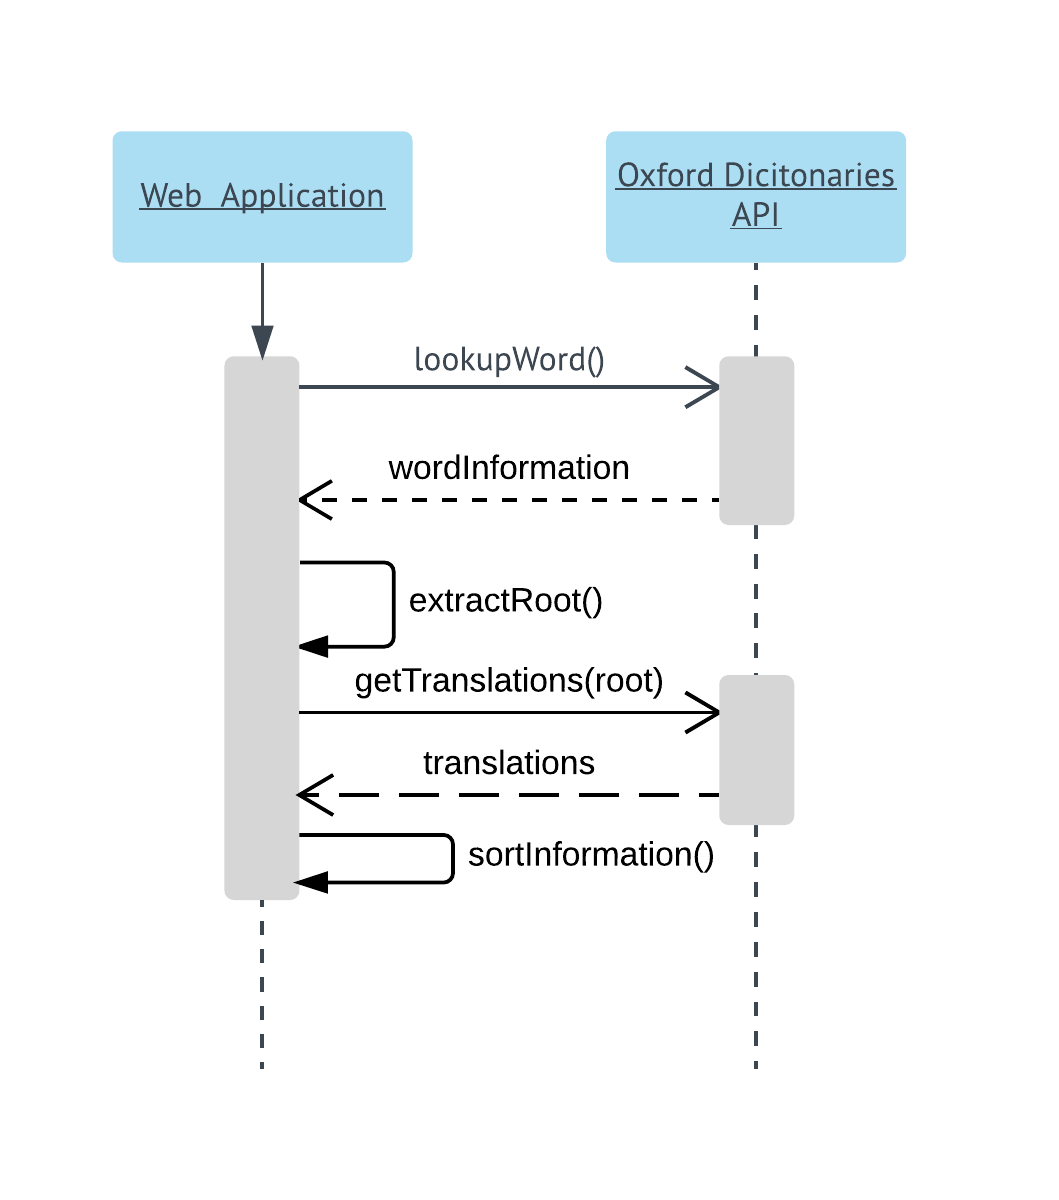
\includegraphics[width=0.7\textwidth]{Graphics/SystemsFlowOxford}
\end{center}
\end{figure}

On the first call, the root word, as provided by \textit{SpaCy}, gets its translations looked up. If one or more translation is discovered, the second call gets made, extracting the grammatical information which lists possible reasons why the root was transformed into its current form.

Several times throughout the grammatical feature generation and translation extraction, the results of \textit{Oxford Dictionaries API} had to be parsed in interesting ways. 

On the first call, there was the problem of extracting the English translations of a word. When translations of a word are looked up using the API, it presents the results as a series of nested lists.  The first of these is a list of 'lexical entries', words with the same spelling but different lexical categories, so the one with the same lexical category as provided by \textit{SpaCy} is used. In this 'lexical entry' there may be one or more 'entries', which are the various homonyms of that spelling. From there an 'entry' may have one or more 'senses' which are the various ways the word can be used. Each 'sense' may then have its own set of 'translations' and these are the translations of the word which are required for the gloss. As every one of these 'translations' in the correct 'lexical entry' is a correct translation of the word provided, they must all be extracted, meaning that every 'entry', 'sense' and 'translation' in the 'lexical entry' has to be iterated through. In addition any one of these lists may not actually be provided, so 'entries' without 'senses' and the like have to be skipped over. The code for this is shown in Listing \ref{lst:eng}. 

\begin{lstlisting}[caption={[Translation Extraction Code] Python code for obtaining the translations of a word from the information provided by the \textit{Oxford Dictionaries API}}, label=lst:eng, breaklines=true, language=python, breakatwhitespace=true, float]
    # iterate through the uses of a word, looking for translations
    @staticmethod
    def sort_english(entries):
        en = []
        for entry in entries:
            if 'senses' in entry.keys():
                senses = entry['senses']
                for sense in senses:
                    if 'translations' in sense.keys():
                        translations = sense['translations']
                        for translation in translations:
                            en.append(translation['text'])
        return en

\end{lstlisting}


More complex was how the API presented grammatical features. All grammatical features from all possible use cases are truncated into a list, so these need to be reassembled into the use cases. An attempt was made to do this and the code for this can be seen in Listing \ref{lst:gramm}.

\begin{lstlisting}[caption=Grammatical Features Extraction Code, label=lst:gramm, breaklines=true, language=python]
@staticmethod
def sort_grammar(gram_fe):
    counter = {}
    # count the occurrences of each grammatical type
    for feature in gram_fe:
        g_type = feature['type'].lower()
        if g_type in counter.keys():
            counter[g_type] += 1
        else:
            counter[g_type] = 1
    # determine the maximum
    if counter == {}:
        return []
    maximum = max(counter, key=(lambda key: counter[key]))
    # create the empty dictionaries
    sorted = [{} for _ in range(counter[maximum])]

    # create another dictionary to keep track of how many times a type has occurred while sorting.
    occurred = {}
    for key in counter.keys():
        occurred[key] = 0

    # sort the features
    for i in range(len(gram_fe)):
        g_type = gram_fe[i]['type'].lower()
        text = gram_fe[i]['text'].lower()
        o = occurred[g_type]
        sorted[o][g_type] = text
        if o == counter[g_type] - 1:
            for j in range(o, len(sorted)):
                sorted[j][g_type] = text
        occurred[g_type] += 1

    # some stuff that has to be coded manually
    if 'person' in sorted[0].keys() and 'number' in sorted[0].keys() and len(sorted) >= 2:
        if sorted[0]['person'] == 'second' and sorted[1]['person'] == 'third':
            sorted[0]['person'] = 'third'
            sorted[1]['person'] = 'second'

    if 'degree' in sorted[0].keys() and len(sorted) > 1:
        if sorted[0]['degree'] == 'positive' and sorted[1]['degree'] == 'comparative':
            sorted[0]['degree'] = 'comparative'
            sorted[1]['degree'] = 'positive'

    return sorted
\end{lstlisting}


The code starts by counting the occurrences of each type of grammatical feature, using the maximum of those counts to calculate the number of use cases there will be. Once it's done that, it iterates through the various features, assigning the n\textsuperscript{th} occurrence of each type to the n\textsuperscript{th} use case. If there are more use cases than occurrences of that type of grammatical feature, the last occurrence is used for the remaining use cases. Finally, there are two sets of use cases that were discovered to be wrong during development and therefore have code written to fix them. 

With the translations and grammatical information extracted, the information can then be given to the gloss generation code from Listing \ref{lst:dict}. 
